For each non-fixed and non-defined variable $x_i$ a propagation queue $q_i$ is made. A propagation queue $q_i$ is an 
topological sort of invariants that are reachable from the vertex representing $x_i$ in the dependency directed 
graph $G$ \boste{maybe define topo sort}. The propagation queue $q_i$ is used such that each invariant dependent on the 
value of $x_i$ is updated at most once if the variable changes value. The DDG show which invariant that are 
directly affected by a change in variable $x_i$ but not the order in which they should be updated. The following example 
show the necessity of such an ordering. 
\begin{center}
    \begin{tikzpicture}[scale=1]
        \vertex[label=$x_1$](x1) at (0,2) {};
        \vertex[label=$i_2$](i2) at (2,1) {};
        \vertex[label=$i_1$](i1) at (4,2) {};
        %\vertex[label=$i_3$](i3) at (5,1) {};
         %\vertex[label=$c_2$](c2) at (5,0) {};
    \tikzset{EdgeStyle/.style={->}}
        \Edge(x1)(i1)
        \Edge(x1)(i2)
        \Edge(i2)(i1)
        %\Edge(x1)(c3)
        %\Edge(y1)(c3)
        %\Edge(y2)(c3)
    \end{tikzpicture}
\end{center}
If $i_1$ is updated before $i_2$ then it might need to be updated again after $i_2$ is updated hence updated twice. In 
worst case updating $x_i$ could lead to a exponential number of updates instead of linear, in the number of vertices 
reachable from $x_i$. \\ 
Once the dependency directed graph is a DAG each invariant vertex has been given a time stamp by Tarjans algorithm. 
Propagation queues are implemented as red-black trees without duplicates hence they have insert time complexity 
$O(log(n))$. For each variable vertex $x_i$ in dependency digraph $G$ a depth first search is made and each vertex 
visited is added to the propagation queue of $x_i$ \boste{currently revisits vertices and adding vertices pointed to 
agian. Should be fixed}. The vertices in the propagation queue are ordered according to their time stamp in decreasing 
order which is a topological sorting such that there is no backward pointing arc. \medskip \\ 
During local search when a single variable $x_i$ changes value the change propagate through the DDG using 
the ordering from the propagation queue $q_i$. When two or more variable changes value the propagation queues are 
merged into a single queue removing duplicates.  